\documentclass{article}
\usepackage{amsmath}
\usepackage{amsfonts}
\usepackage{graphicx}
\usepackage{siunitx}
\usepackage{booktabs}
\usepackage{tikz}
\usepackage{pgfplots}
\usepackage{geometry}
\geometry{a4paper, margin=2.5cm}
\pgfplotsset{compat=1.18}

\title{Rekonstruktive Spektralformel der Beta-Skala}
\author{}
\date{}

\begin{document}

\maketitle

\section*{1. Rekonstruktive Näherung für \boldmath$\beta_k$}

Die rekonstruktive Formel basiert auf der spektralen Zerlegung der Fehlerfunktion \(\varepsilon(n)\). Die Beta-Skala entsteht durch gewichtete Cosinus-Oszillationen dominanter Frequenzanteile:

\[
\beta_k \approx \sum_{n=1}^{N} \frac{A_n}{k^\delta} \cdot \cos\left(2\pi f_n \cdot \log(k) + \varphi_n \right)
\]

\noindent\textbf{Parameter:}
\begin{itemize}
  \item \(k \in \mathbb{N}\): Position in der Beta-Folge
  \item \(f_n\): Frequenzanteile (s. Tabelle)
  \item \(A_n\): zugehörige Amplituden
  \item \(\varphi_n \approx 0\): Phasen (typisch ignoriert)
  \item \(\delta > 0\): Dämpfung zur Konvergenzsteuerung
\end{itemize}

\section*{2. Dominante Frequenzen aus dem Spektrum von \boldmath$\varepsilon(n)$}

\begin{table}[h!]
\centering
\begin{tabular}{@{}rr@{}}
\toprule
\textbf{Frequenz \( f_n \)} & \textbf{Amplitude \( A_n \)} \\
\midrule
9.994743e-06 & 1.82e+08 \\
9.495006e-06 & 1.91e+08 \\
8.995268e-06 & 2.00e+08 \\
8.495531e-06 & 2.11e+08 \\
7.995794e-06 & 2.23e+08 \\
7.496057e-06 & 2.36e+08 \\
6.996320e-06 & 2.51e+08 \\
6.496583e-06 & 2.68e+08 \\
5.996846e-06 & 2.87e+08 \\
5.497109e-06 & 3.09e+08 \\
4.997371e-06 & 3.35e+08 \\
4.497634e-06 & 3.66e+08 \\
3.997897e-06 & 4.03e+08 \\
3.498160e-06 & 4.47e+08 \\
2.998423e-06 & 5.02e+08 \\
2.498686e-06 & 5.70e+08 \\
1.998949e-06 & 6.54e+08 \\
9.994743e-07 & 7.44e+08 \\
1.499211e-06 & 7.45e+08 \\
4.997371e-07 & 1.30e+09 \\
\bottomrule
\end{tabular}
\caption{Top 20 Frequenzanteile mit zugehörigen Amplituden aus dem Fourier-Spektrum von \(\varepsilon(n)\).}
\end{table}

\section*{3. Schematische Visualisierung: Cosinus-Summe}

\begin{figure}[h!]
\centering
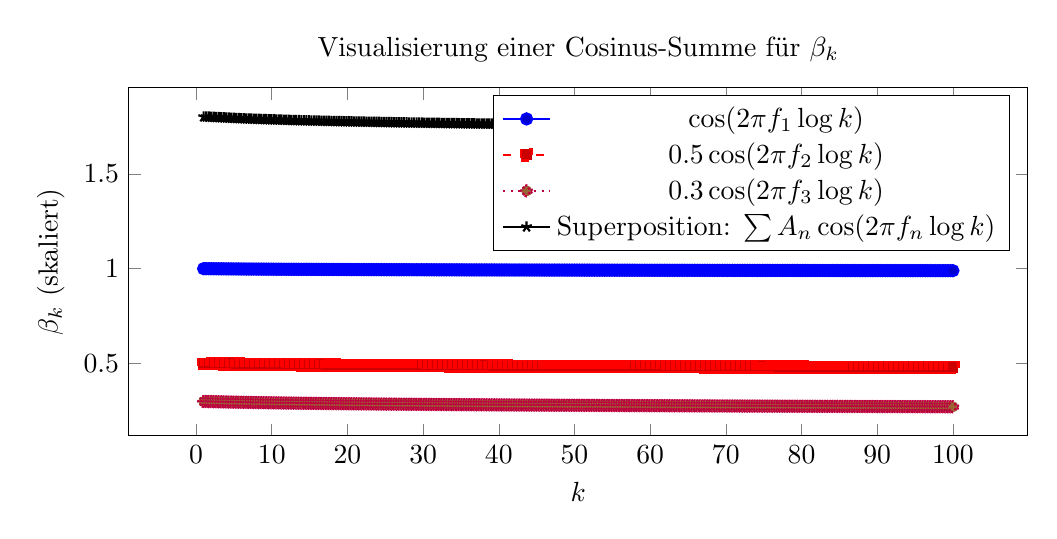
\begin{tikzpicture}
\begin{axis}[
    width=13cm, height=6cm,
    xlabel={$k$}, ylabel={$\beta_k$ (skaliert)},
    title={Visualisierung einer Cosinus-Summe für $\beta_k$},
    domain=1:100, samples=300,
    legend style={at={(0.98,0.98)}, anchor=north east}
]
\addplot+[blue, thick] {cos(deg(2*pi*0.005*ln(x)))};
\addlegendentry{$\cos(2\pi f_1 \log k)$}

\addplot+[red, thick, dashed] {0.5*cos(deg(2*pi*0.01*ln(x)))};
\addlegendentry{$0.5\cos(2\pi f_2 \log k)$}

\addplot+[purple, thick, dotted] {0.3*cos(deg(2*pi*0.015*ln(x)))};
\addlegendentry{$0.3\cos(2\pi f_3 \log k)$}

\addplot+[black, thick, domain=1:100, samples=300] 
{cos(deg(2*pi*0.005*ln(x))) + 0.5*cos(deg(2*pi*0.01*ln(x))) + 0.3*cos(deg(2*pi*0.015*ln(x)))};
\addlegendentry{Superposition: $\sum A_n \cos(2\pi f_n \log k)$}
\end{axis}
\end{tikzpicture}
\caption{Skalierte Cosinus-Summe als schematische Näherung der rekonstruktiven Beta-Skala.}
\end{figure}

\end{document}